%%%%%%%%%%%%%%%%%%%%%%% file template.tex %%%%%%%%%%%%%%%%%%%%%%%%%
%
% This is a general template file for the LaTeX package SVJour3
% for Springer journals.          Springer Heidelberg 2010/09/16
%
% Copy it to a new file with a new name and use it as the basis
% for your article. Delete % signs as needed.
%
% This template includes a few options for different layouts and
% content for various journals. Please consult a previous issue of
% your journal as needed.
%
%%%%%%%%%%%%%%%%%%%%%%%%%%%%%%%%%%%%%%%%%%%%%%%%%%%%%%%%%%%%%%%%%%%
%
% First comes an example EPS file -- just ignore it and
% proceed on the \documentclass line
% your LaTeX will extract the file if required
\begin{filecontents*}{example.eps}
%!PS-Adobe-3.0 EPSF-3.0
%%BoundingBox: 19 19 221 221
%%CreationDate: Mon Sep 29 1997
%%Creator: programmed by hand (JK)
%%EndComments
gsave
newpath
  20 20 moveto
  20 220 lineto
  220 220 lineto
  220 20 lineto
closepath
2 setlinewidth
gsave
  .4 setgray fill
grestore
stroke
grestore
\end{filecontents*}
%
\RequirePackage{fix-cm}
%
%\documentclass{svjour3}                     % onecolumn (standard format)
%\documentclass[smallcondensed]{svjour3}     % onecolumn (ditto)
\documentclass[smallextended]{svjour3}       % onecolumn (second format)
%\documentclass[twocolumn]{svjour3}          % twocolumn
%
\smartqed  % flush right qed marks, e.g. at end of proof
%

\usepackage{graphicx}
\usepackage{amsmath}
\usepackage{algorithm}
\usepackage{algorithmic}
\renewcommand{\algorithmicrequire}{\textbf{Initialize:}}

\usepackage{verbatim} %TODO delete before submission
\usepackage[numbers]{natbib}%TODO delete before submission

%TODO Zitierweise ändern, sieht schrecklich aus
%
% \usepackage{mathptmx}      % use Times fonts if available on your TeX system
%
% insert here the call for the packages your document requires
%\usepackage{latexsym}
% etc.
%
% please place your own definitions here and don't use \def but
% \newcommand{}{}
%
% Insert the name of "your journal" with
% \journalname{myjournal}
%
\begin{document}

\title{Extensions for DDPG and analysis of its components
%\thanks{Grants or other notes
%about the article that should go on the front page should be
%placed here. General acknowledgments should be placed at the end of the article.}
}
\subtitle{subtitle here}

%\titlerunning{Short form of title}        % if too long for running head

\author{Yannik Frisch \and Tabea Wilke \and Maximilian Gehrke %etc.
}

%\authorrunning{Short form of author list} % if too long for running head

\institute{F. Author \at
              first address \\
              Tel.: +123-45-678910\\
              Fax: +123-45-678910\\
              \email{fauthor@example.com}           %  \\
%             \emph{Present address:} of F. Author  %  if needed
           \and
           S. Author \at
              second address
}

\date{Received: date / Accepted: date}
% The correct dates will be entered by the editor


\maketitle

\begin{abstract}
TODO
\keywords{DDPG \and DQN \and DPG}
% \PACS{PACS code1 \and PACS code2 \and more}
% \subclass{MSC code1 \and MSC code2 \and more}
\end{abstract}

\section{Introduction}
\label{sec:intro}
Deep Deterministic Policy Gradients (DDPG) arises from Deterministic Policy 
Gradients (DPG) and Deep Q-Learning (DQN). In the following we describe the 
underlying algorithms DPG and DQN and which aspects DDPG uses of both of them. 

\subsection{Deep Q-Learning (DQN) }
\nocite{mnih2015human}
\nocite{mnih2013playing}
\label{sec:DQN}
The DQN approach combines the approximation power of Neural Networks with traditional Q-learning.
It enables solving the classic Reinforcement Learning problem of achieving the maximum expected reward over time, even for large state spaces (e.g. image frames). The algorithm is an off-policy, model-free approach and is able to find a close to optimal action-value function for many cases [x] and from this a close to optimal deterministic policy by greedily selecting the action: $\pi(s)=\max_{a}Q^*(s,a)$. In terms of a formula the optimal action-value function is represented by
\[ 
Q^*(s_t,a_t)=\max_\pi E \left[
\sum_{t^{'}=t}^{T}\gamma^{t^{'}-t}r_{t^{'}}|s_t=s,
a_t=a, \pi \right] 
\]
%TODO E richtig darstellen
 where $\gamma\in[0,1)$ is called the discount factor, controlling the agents preference for rewards closer or further away in time. Rewards later on in an episode will still have impact on the result but their influence decreases by the amount of time-steps required to reach them in the future.
By definition this optimal value function yields the Bellman equation [x] and can be reinterpreted as maximizing the current reward and the discounted action-value of the resulting state. In formula this gives:
\[
Q^*(s,a) = E_{s'\sim\epsilon}\left[
r + \gamma \max_{a'}Q^*(s',a')|s,a \right]
\]
%TODO E
For approximating the action-value function $Q(s,a|\theta)\approx Q^*(s,a)$ the approach uses a deep neural network, called the Q-Network.
The Q-Network can be trained by minimizing a sequence of loss functions $L_i(\theta_i)$, depending on it's weights:
\[
L_i(\theta_i)=E_{s,a\sim\rho(.),s'\sim\epsilon}
\left[\left(r+\gamma \max_{a'} Q(s', 
a'|\theta_{i-1})-Q(s,a|\theta_i)\right)^2\right] 
\]
%TODO E richtig machen
This loss function is similiar to the classical temporal-difference loss used in Q-Learning, but with approximated action-value functions instead of lookup-tables. Derivating this loss w.r.t. the approximation's weights gives:
\[
\nabla_{\theta_i}L_i(\theta_i)=E_{s,a\sim\rho(.),s'\sim\epsilon}
\left[\left(r+\gamma \max_{a'} Q(s', 
a'|\theta_{i-1})-Q(s,a|\theta_i)\right)\nabla_{\theta_i}Q(s,a|\theta_i)\right] 
\]
This gradient can be used to optimize the loss function by using stochastic gradient descent.\\
Furthermore, a replay buffer is used which stores samples of the environment. This allows random mini-batch sampling, which decorrelates the samples and is proven to improve the performance by greater data efficiency [x]. The mini-batch sampling also enables the use of improved derivatives of vanilla stochastic gradient descent, e.g. RPROP as in the 'neural fitted Q-Learning (NFQ)' [x] approach or ADAM update [x].\\
%TODO Rewrite the target network stuff
There are different ways of estimating the expected Q-values. Either with a target network with the same structure as the network for the action-value function or the normal network. If a target network is used, the target weights need to be updated after some 
training steps.\\
A pseudocode for the DQN approach can be found in \ref{DQN-algo}.
The DQN approach was able to significantly outperform earlier learning methods despite incorporating almost no prior knowledge about the inputs [x], but is limited by the disabilty to cope with continous and high-dimensional action spaces due to the max operator in the action selection [x]. This limitations can be adressed by combining the approach with the Deterministic Policy Gradient, which is described in the following section.

\begin{algorithm}
	\caption{Deep Q-Learning (DQN)}\label{DQN-algo}
	\begin{algorithmic}
		\REQUIRE Replay buffer $\mathit{D}$ with high capacity
		\REQUIRE Neural network for action-value function $\mathit{Q}$
		with random weights $\theta$
		\REQUIRE Neural network for target action-value function$
		\mathit{\hat{Q}}$ with weights $\theta^-=\theta$
		\FOR{episode $1$ \TO $M$}
		\STATE reset environment to state $s_1$
		\FOR{$t=1$ \TO $T$}
		\IF{random $i \le \epsilon$}
		\STATE random action $a_t$
		\ELSE
		\STATE $a_t=\operatorname*{argmin}_a Q(s_t,a|\theta)$
		\ENDIF
		\STATE execute $a_t \rightarrow$ reward $r_t$ and next state 
		$s_{t+1}$
		\STATE save $(s_t, a_t, r_t,s_{t+1})$ in $D$
		\STATE sample minibatch $(s_i, a_i, r_i,s_{i+1})$ from $D$
		\STATE $q_i =
			\begin{cases}
			r_i & \textit{if episode terminates at step i+1}\\
			r_i+\gamma \max_{a'}\hat{Q}(s_{i+1}, a'|\theta^{-})& 
			else\\			
			\end{cases}$
		\STATE perform gradient descent on $\left(q_i-Q\left(s_i, 
		a_i|\theta\right)\right)^2_\theta$
		\STATE every $C$ steps update $\hat{Q}=Q$
		\ENDFOR
		\ENDFOR
	\end{algorithmic}
\end{algorithm}


\subsection{Deterministic Policy Gradient (DPG)}
\label{sec:DPG}
\nocite{lillicrap2015continuous}
Most problems in reinforcement learning consist of a continuous action space which makes it very difficult to greedily choose the best action given a policy, due to the max operator. From a stochastic point of view, the policy is a probability distribution $a\sim\pi(a|s)$ over all actions. In order to calculate the gradient of a parameterized policy $\pi(a,s|\theta)$ over the total reward w.r.t. the weights, one needs to solve an integral over all actions, which becomes untractable for large action spaces.\\
From a deterministic view the policy is a discrete mapping from states to actions $a=\pi(s)$ and thus only one integration over the state space is sufficient. The \textit{policy gradient theorem} [x] gives the update rule for a parameterized deterministic policy function $\pi(s|\theta)$:
%TODO Get from DPG paper to this update rule
\begin{align*}
\nabla_{\theta^\pi}J
&\approx E_{s_t\sim\rho^\beta}\left[\nabla_{\theta^\pi}Q(s,a|\theta^Q)\right] \\
&= E_{s_t\sim\rho^\beta}\left[\nabla_aQ(s,a|\theta^Q)|_{s=s_t,a=\pi(st)} \nabla_{\theta^\pi}\pi(s|\theta^\pi)|_{s=s_t}\right]
\end{align*}
where the expectation can again be obtained from sampling from an environment.


The integration is done via importance sampling. As a result of this, stochastic policy gradients need much more samples than deterministic policy gradients. To handle the exploration-exploitation dilemma, the idea of \citeauthor{silver2014deterministic} is to use a stochastic behaviour policy and a deterministic target policy. The behaviour policy should ensure that the exploration is big enough and the target policy should exploit enough based on 
the policy gradient. The algorithm they used was an off-policy actor-critic method. Thereby, the action-value function is estimated with a function approximation. The policy parameters will be updated in direction of the gradient of the action-value function. The direction of the gradient underlies 
the \textit{policy gradient theorem}: 

\begin{align*}
\bigtriangledown_\theta 
J(\pi_\theta)&=\int_{S}^{}\rho^\pi(s)\int_{A}\bigtriangledown_\theta 
\pi_\theta(a|s)Q^\pi(s,a)\mathrm{d}a\mathrm{d}s\\
&=E_{s \sim \rho^\pi,\: a\sim\pi_\theta}[\bigtriangledown_\theta \log 
\pi_\theta (a|s)Q^\pi(s,a)]
\end{align*}%TODO E richtig darstellen (\mathbb{})

\subsection{Actor-Critic Methods}
\label{sec:actor-critic}
The advantage of actor-critic methods is that they learn policies as well as 
value functions. To get an intuition about these methods the following figure 
illustrates the update-cycle:
\begin{figure}[H]
	\centering
	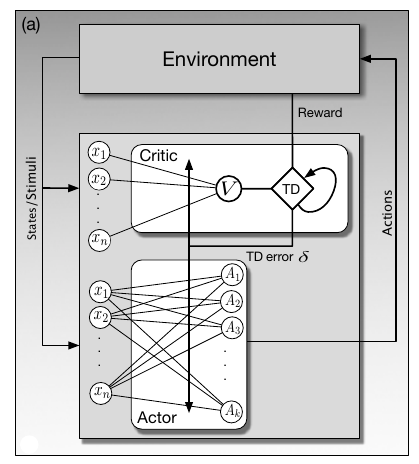
\includegraphics[width=0.4\linewidth]{actor-critic}
	\caption{Intuition about actor-critic methods (figure from 
	\cite{sutton2018reinforcement})}
	\label{fig:actor-critic}
\end{figure}
The actor is responsible for the change of the policies, the critic has to 
update the parameter of the state-value function. Updating the actors' and the 
critics' parameter follows the TD-error of the critic which is produced through 
the reward and the current error of the estimated state values. As Fig. 
\ref{fig:actor-critic} illustrates, the actor has no information about the 
current reward and the critic has no direct influence on the actions.  
%TODO direct influence richtig formuliert?
The update of actor and critic can be formulated as follows:
\begin{figure}[H]
	\centering
	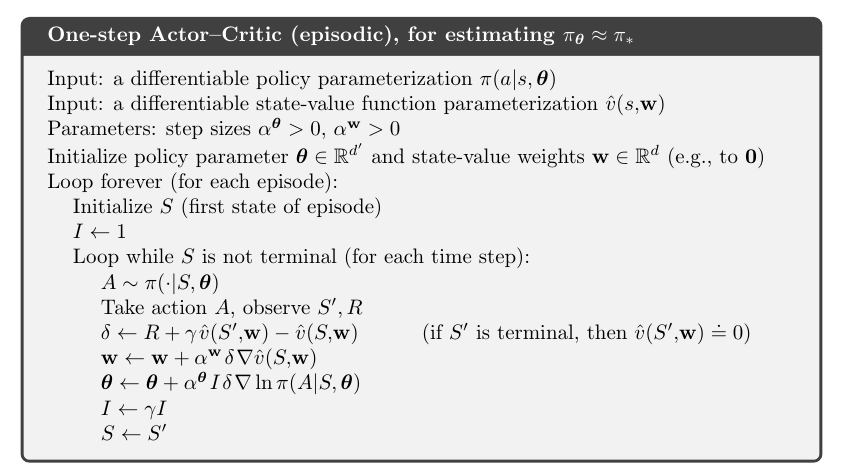
\includegraphics[width=0.6\linewidth]{actor-critic-algo}
	\caption{Intuition about actor-critic methods (figure from 
		\cite{sutton2018reinforcement})}
	\label{fig:actor-critic-algo}
\end{figure}
%TODO if we want it, change it to self written

\subsection{Deep Deterministic Policy Gradient (DDPG)}
\nocite{lillicrap2015continuous}
The combination of above approaches leds to the \textit{Deep Deterministic Policy Gradient (DDPG)} approach, which is a model-free and off-policy algorithm. It can be grouped into the class of policy gradient algorithms and uses actor-critic methods with a deterministic target policy and deep Q-learning. Both, the actor and the critic, are realized by deep neural networks. The pseudocode for DDPG can be found in \ref{DDPG-algo}.
%TODO Add refference
\begin{algorithm}
	\caption{Deep Deterministic Policy Gradient (DDPG)}\label{DDPG-algo}
	\begin{algorithmic}
		\REQUIRE Replay buffer $\mathit{D}$ with high capacity
		\REQUIRE Initialize critic network $Q(s,a|\theta^Q)$ and actor network $\pi(s|\theta^\pi)$ with random weights $\theta^Q$ and $\theta^\pi$
		\REQUIRE Initialize target networks $Q'$ and $\pi'$ with weights $\theta^{Q'}\leftarrow\theta^Q$ and $\theta^{\pi'}\leftarrow\theta^\pi$
		\FOR{episode $1$ \TO $M$}
		\STATE Initialize random process $\mathit{N}$ for action exploration
		\STATE Reset environment to state $s_1$
		\FOR{$t=1$ \TO $T$}
		\STATE Select action $a_t = \pi(s_t|\theta^\pi) + \mathit{N}_t$ from local actor
		\STATE Execute action $a_t$ and observe reward $r_t$ and next state $s_{t+1}$
		\STATE Save $(s_t, a_t, r_t,s_{t+1})$ in replay buffer $D$
		\STATE Sample minibatch $(s_i, a_i, r_i,s_{i+1})$ from $D$
		\STATE Set TD-target from target networks:\\
		\qquad $y_i = r_i + \gamma Q'(s_{i+1}, \pi'(s_{i+1}|\theta^{\pi'})|\theta^{Q'})$
		\STATE Update the critic by minimizing the loss:\\
		\qquad $L=\frac{1}{N}\sum_i(y_i - Q(s_i,a_i|\theta^Q))^2$
		\STATE Update the actor using the sampled policy gradient:\\ 			\qquad $\nabla_{\theta^\pi}J \approx \frac{1}{N} \sum_i \nabla_a Q(s,a|\theta^Q)|_{s=s_i, a=\pi(s_i)}\nabla_{\theta^\pi}\pi(s|\theta^\pi)|_{s=s_i}$
		\STATE Update the target networks:\\
		\qquad $\theta^{Q'}\leftarrow \tau \theta^Q + (1-\tau)\theta^{Q'}$\\
		\qquad $\theta^{\pi'}\leftarrow \tau \theta^\pi + (1-\tau)\theta^{\pi'}$
		\ENDFOR
		\ENDFOR
	\end{algorithmic}
\end{algorithm}
\\
\\
\begin{itemize}
\item DQN uses deep networks to estimate the action-value function
\begin{itemize}
\item it can only handle discrete and low-dim action spaces
\end{itemize}
\item discretizing the action space often suffers from the course of dimensionality
\item PolicyGradientTheorem from continous space to discrete space presented in DPG paper
\item naive extension of DPG with nns turns out to be unstable for challenging problems
\item Deep DPG (DDPG): combination of DQN and DPG, where:
\begin{itemize}
\item networks are trained off-policy with samples from a replay buffer to minimize the temporal correlations between samples
\item the networks are trained with target networks to give consistent targets during temporal difference backups
\item batch normalization is used
\end{itemize}
\item DDPG is able to learn from low dim observations (torques etc.), aswell as from high dim observations in pixel space
\end{itemize}


\section{Extensions to the Algorithm}
\label{sec:1}
\begin{comment}

We propose several possible extensions and show their performance on a task.\\
Text with citations \cite{RefB} and \cite{RefJ}.
\subsection{Subsection title}
\label{sec:2}
as required. Don't forget to give each section
and subsection a unique label (see Sect.~\ref{sec:1}).
\paragraph{Paragraph headings} Use paragraph headings as needed.
\begin{equation}
a^2+b^2=c^2
\end{equation}

% For one-column wide figures use
\begin{figure}
% Use the relevant command to insert your figure file.
% For example, with the graphicx package use
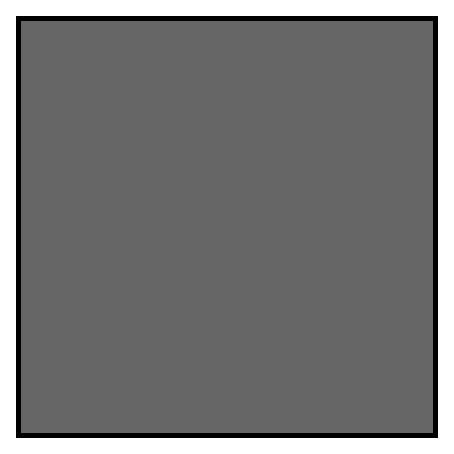
\includegraphics{example.eps}
% figure caption is below the figure
\caption{Please write your figure caption here}
\label{fig:1}       % Give a unique label
\end{figure}
%
% For two-column wide figures use
\begin{figure*}
% Use the relevant command to insert your figure file.
% For example, with the graphicx package use
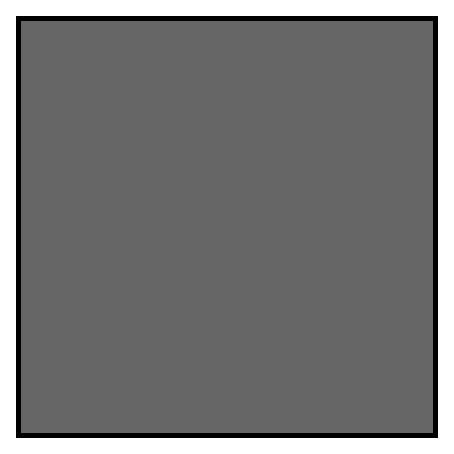
\includegraphics[width=0.75\textwidth]{example.eps}
% figure caption is below the figure
\caption{Please write your figure caption here}
\label{fig:2}       % Give a unique label
\end{figure*}


%
% For tables use
\begin{table}
% table caption is above the table
\caption{Please write your table caption here}
\label{tab:1}       % Give a unique label
% For LaTeX tables use
\begin{tabular}{lll}
\hline\noalign{\smallskip}
first & second & third  \\
\noalign{\smallskip}\hline\noalign{\smallskip}
number & number & number \\
number & number & number \\
\noalign{\smallskip}\hline
\end{tabular}
\end{table}


\end{comment}
%\begin{acknowledgements}
%If you'd like to thank anyone, place your comments here
%and remove the percent signs.
%\end{acknowledgements}

% BibTeX users please use one of
\bibliographystyle{spbasic}      % basic style, author-year citations
%\bibliographystyle{spmpsci}      % mathematics and physical sciences
%\bibliographystyle{spphys}       % APS-like style for physics
\bibliography{ddpg.bib}   % name your BibTeX data base

% Non-BibTeX users please use
\begin{comment}


\begin{thebibliography}{}
%
% and use \bibitem to create references. Consult the Instructions
% for authors for reference list style.
%
\bibitem{RefJ}
% Format for Journal Reference
Author, Article title, Journal, Volume, page numbers (year)
% Format for books
\bibitem{RefB}
Author, Book title, page numbers. Publisher, place (year)
% etc

\end{thebibliography}
\end{comment}
\end{document}
% end of file template.tex
